\documentclass[conference,a4paper]{IEEEtran}
% IEEEtran provides the IEEE layout: two columns, 10 pt Times, section headings
% ("I. INTRODUCTION", "A. Subsection"), "Fig." and "TABLE I" captions, and
% references to subsections printed as "Section III-A".

% ----------------------------------------------------------------- Fonts
\usepackage[T1]{fontenc}
\usepackage[utf8]{inputenc}
% Times text and math. newtx is preferred; mathptmx is a fallback that ships
% with every TeX distribution.
\IfFileExists{newtxtext.sty}
  {\usepackage{newtxtext}\usepackage{newtxmath}}
  {\usepackage{mathptmx}\usepackage{amssymb}}   % amssymb: \mathbb (newtxmath has it built in)
\usepackage{microtype}
% Long file names in \texttt cannot be hyphenated; allow a little extra
% inter-word space instead of letting them stick out into the margin.
\setlength{\emergencystretch}{2em}

% ---------------------------------------------------------------- Content tools
\usepackage{amsmath}
\interdisplaylinepenalty=2500   % recommended by IEEEtran when using amsmath
\usepackage{graphicx}
\usepackage{booktabs}
\usepackage{array}
\usepackage{enumitem}
\usepackage{listings}
\usepackage{xcolor}
\usepackage{balance}   % equal-height columns on the last page (IEEE style)

% Figures generated by assignment_1/plot_results.py. They are designed for a
% 3.5 in column, so \includegraphics[width=\columnwidth] prints them at the
% intended size (see common/plotting_style.md).
\graphicspath{{../results/}}

% Code listings (small, monospaced, light frame).
\lstset{basicstyle=\footnotesize\ttfamily, frame=lines, framesep=3pt,
        columns=fullflexible, keepspaces=true, xleftmargin=0pt, xrightmargin=0pt}

% Links in the deep blue used for C in the figures.
\definecolor{linkblue}{HTML}{1F43B2}
\usepackage[colorlinks=true,linkcolor=linkblue,citecolor=linkblue,urlcolor=linkblue]{hyperref}
\hypersetup{pdftitle={Basic Matrix Multiplication in Different Languages (C, Java \& Python)},
            pdfauthor={Javier Ruano Hernández}}

% ------------------------------------------------------------- Placeholders
% \TODO{...} prints a red marker in the PDF so no placeholder is forgotten.
\newcommand{\TODO}[1]{\textcolor{red}{\textbf{[TODO: #1]}}}

% ------------------------------------------------------------------ Shortcuts
\newcommand{\bigO}[1]{\mathcal{O}\!\left(#1\right)}
\newcommand{\code}[1]{\texttt{#1}}

% =============================================================================
\title{Basic Matrix Multiplication in Different Languages\\(C, Java \& Python)}
\author{\IEEEauthorblockN{Javier Ruano Hernández}
\IEEEauthorblockA{Big Data -- Assignment 1\\
Universidad de Las Palmas de Gran Canaria (ULPGC)\\
% Check that the repository is public (or that the instructor has access).
Code and data: \url{https://github.com/javierruanohdez/big-data-assignments/tree/main/assignment_1}}}

\begin{document}
\maketitle

% =============================================================================
% ABSTRACT
% =============================================================================
\begin{abstract}
This report studies how the matrix size $n$ affects the execution time and the
memory usage of the textbook $\bigO{n^3}$ dense matrix multiplication algorithm,
implemented with the same triple loop in C, Java and Python. All three
implementations use 64-bit floating-point numbers, the same flat row-major
memory layout and bit-identical input matrices read from a shared binary file.
They are validated against a correctly rounded reference before benchmarking.
For $n \in \{100, 250, 500, 1000\}$, each configuration was run five times in
fresh processes, timing only the multiplication kernel with a monotonic clock
and recording the peak resident set size.
On the tested machine, the empirical time-scaling exponents were 3.30 (C),
2.84 (Java) and 3.27 (Python), close to the cubic model. At $n=1000$, the median
kernel time was 1.46~s in C, 1.61~s in Java and 103.8~s in Python. At the same
size, peak memory was 24.8~MB in C, close to the 22.9~MB occupied by the three
matrices, but 4.3 times that size in Java and 5.7 times in Python because of
runtime overhead. These results describe one machine and one configuration and
are not general claims about the languages.
\end{abstract}

\begin{IEEEkeywords}
matrix multiplication, benchmarking, performance evaluation, JIT compilation,
interpreters, memory hierarchy.
\end{IEEEkeywords}

% =============================================================================
\section{Introduction and Objective}
\label{sec:intro}
% =============================================================================

Dense matrix multiplication is one of the most fundamental kernels in
computing: it is at the core of numerical linear algebra, scientific
simulation, machine learning and many data-processing pipelines. The textbook
algorithm computes each element of $C = AB$ as a dot product of a row of $A$
and a column of $B$. For $n \times n$ matrices it performs $2n^3$ floating-point
operations and stores $3n^2$ values. This gives a simple model: execution time
should grow as $n^3$ and memory as $n^2$.

In practice, the measured cost of the same algorithm depends heavily on how it
is executed. The same triple loop can be compiled ahead of time to native code
(C), compiled at run time by a just-in-time (JIT) compiler (Java) or executed by
a bytecode interpreter (Python). Each execution model adds different overheads
per operation and represents numbers differently in memory. In addition, the
memory hierarchy of modern processors makes the cost of an operation depend on
where its data lives. As a result, real programs can deviate from the
operation-count model.

\paragraph{Objective} The objective of this work is to answer the following
research question:

\begin{quote}
\emph{How does the matrix size $n$ affect the execution time and memory usage of
the basic $\bigO{n^3}$ matrix multiplication when the same algorithm is
implemented in C, Java and Python and run on the same machine?}
\end{quote}

\noindent We split it into three sub-questions:
\begin{enumerate}[label=\textbf{RQ\arabic*.}, leftmargin=3.2em, itemsep=1pt]
  \item How closely does the measured execution time follow the theoretical
        $n^3$ growth in each language?
  \item How does peak memory grow with $n$, compared with the theoretical
        size of the three matrices ($3 \times 8n^2$ bytes)?
  \item How do the execution models (ahead-of-time compilation, JIT compilation,
        interpretation) and memory layouts affect the constant factors?
\end{enumerate}

\paragraph{Contributions} We provide (i)~three implementations that perform
identical arithmetic on identical inputs; (ii)~a reproducible pipeline with a
shared input generator, automated correctness checks, an automated benchmark
harness and scripted analysis; and (iii)~a measurement-based comparison with the
theoretical model. All code and raw data are publicly available in the
repository linked on the first page.

\paragraph{Scope} The results describe a single machine and configuration
(Section~\ref{sec:environment}). They do not support general claims that one
language is faster than another.

The rest of this report is organized as follows. Section~\ref{sec:background}
introduces the algorithm, the memory hierarchy and the execution models.
Section~\ref{sec:method} describes the experimental methodology,
Section~\ref{sec:results} presents the results and Section~\ref{sec:discussion}
discusses them. Section~\ref{sec:conclusions} concludes.

% =============================================================================
\section{Background and References}
\label{sec:background}
% =============================================================================

\subsection{The Triple-Loop Algorithm}
For $A, B \in \mathbb{R}^{n \times n}$, the product $C = AB$ is defined element
by element as
\begin{equation}
  c_{ij} = \sum_{k=0}^{n-1} a_{ik}\, b_{kj}, \qquad 0 \le i, j < n.
  \label{eq:matmul}
\end{equation}
Evaluating \eqref{eq:matmul} directly with three nested loops requires $n^3$
multiplications and $n^3$ additions, so the running time is $\Theta(n^3)$. The
three matrices occupy $3n^2$ values, i.e.\ $24n^2$ bytes in double precision.
Asymptotically faster algorithms exist, starting with Strassen's
$\bigO{n^{2.807}}$ method~\cite{strassen1969}. High-performance libraries
(BLAS implementations) keep the $\bigO{n^3}$ operation count but reorganize
the computation into cache-sized blocks and use vector instructions, reaching a
large fraction of the processor's peak speed~\cite{goto2008}. This assignment
deliberately excludes such optimizations and studies the unoptimized algorithm.

\subsection{Memory Hierarchy and Access Patterns}
Modern processors hide the latency of main memory behind several levels of
cache, which hold recently used data in fixed-size lines, typically 64
bytes~\cite{hennessy2017,drepper2007}. Code that accesses consecutive addresses
uses every byte of each line it loads; code that jumps through memory loads
a full line for every element it uses.

With row-major storage, element $(i,j)$ is at offset $i \cdot n + j$. In the
i-j-k loop order used here, the innermost loop over $k$ reads $A$ along a row
(unit stride, cache-friendly) but reads $B$ down a column (stride of $8n$
bytes). For any practical $n$, each step of the inner loop therefore touches a
different cache line of $B$. These lines can be reused by the next iteration
over $j$ only if all $n$ of them still fit in cache. Once the working set
exceeds a cache level, the number of misses per operation increases. Execution
time can then grow faster than $n^3$ even though the operation count does
not~\cite{lam1991}.

\subsection{Execution Models}
\textbf{C} is compiled \emph{ahead of time} (AOT) to native machine code. The
compiler optimizes the whole program before it runs, and execution adds no
run-time overhead beyond the program itself.

\textbf{Java} is compiled to platform-independent bytecode. The HotSpot JVM
starts by interpreting it and, once a method or loop has run often enough,
compiles it at run time to optimized native code. This happens in tiers: first
the fast C1 compiler, then the optimizing C2 compiler~\cite{paleczny2001}. Long
loops can be switched to compiled code while they run (on-stack replacement).
Steady-state performance can therefore approach that of AOT-compiled code. The
first executions, however, are slower and include compilation time, which is
why Java benchmarks need warm-up runs~\cite{georges2007}.

\textbf{Python} (CPython) compiles source code to bytecode and executes it in an
interpreter loop. Every operation is dispatched at run time with dynamic type
checks. Numbers are heap-allocated objects: a \code{float} object occupies 24
bytes on a 64-bit system, and a \code{list} stores 8-byte pointers to such
objects. Each arithmetic operation in the inner loop therefore costs many
machine instructions and may allocate a new object.

\subsection{Benchmarking and Floating-Point Arithmetic}
Reliable performance measurements require warm-up for managed runtimes,
several repetitions, robust statistics and a clear definition of what is
measured~\cite{georges2007,kalibera2013}. We report medians and interquartile
ranges, which are robust to occasional slow runs.

Finally, IEEE~754 floating-point addition is not associative~\cite{ieee754}.
Different evaluation orders or the use of fused multiply-add instructions can
change the last bits of a result. Results from different implementations must
therefore be compared with tolerances derived from rounding-error
analysis~\cite{higham2002}, not with exact equality.

% =============================================================================
\section{Methodology}
\label{sec:method}
% =============================================================================

\subsection{Experimental Environment}
\label{sec:environment}
All measurements were taken on the machine described in
Table~\ref{tab:environment}, with other applications closed and the computer
connected to mains power.

\begin{table}[t]
  \centering
  \caption{Hardware and software environment}
  \label{tab:environment}
  \footnotesize
  % Sources: lscpu, free, /etc/os-release, uname, Win32_Processor / Win32_PhysicalMemory
  % (PowerShell), wsl --version; core types and boost clocks from the CPU's specification.
  \begin{tabular}{@{}l>{\raggedright\arraybackslash}p{0.64\columnwidth}@{}}
    \toprule
    \textbf{Item} & \textbf{Value} \\
    \midrule
    CPU model                        & AMD Ryzen AI 5 330 (laptop) \\
    Cores / logical threads          & 4 (1$\times$ Zen~5 + 3$\times$ Zen~5c) / 8 \\
    Clock                            & 2.0~GHz base; boost up to 4.5~GHz (Zen~5), 3.4~GHz (Zen~5c) \\
    Caches                           & L1d 48~KB and L2 1~MB per core; L3 8~MB shared \\
    RAM                              & 32~GB LPDDR5X-8000 (15~GB available to WSL~2) \\
    Operating system                 & Windows 11 Home (build 26200), WSL 2.7.14, Ubuntu 26.04 LTS \\
    Kernel                           & 6.18.33.2-microsoft-standard-WSL2 \\
    C compiler                       & GCC 15.2.0 \\
    Java runtime                     & OpenJDK 25.0.4.1 (Ubuntu build) \\
    Python                           & CPython 3.14.4 \\
    Analysis                         & pandas 3.0.5, Matplotlib 3.11.2 \\
    \bottomrule
  \end{tabular}
\end{table}

\subsection{Implementations}
The three implementations (\code{matmul.c}, \code{MatMul.java},
\code{matmul.py}) follow the same structure: load the inputs, multiply, report.
To keep the comparison fair, they share every algorithmic decision:
\begin{itemize}[itemsep=1pt]
  \item the same \textbf{i-j-k loop order}, the direct translation of
        \eqref{eq:matmul} (Listing~\ref{lst:kernel});
  \item a \textbf{local accumulator} for each dot product, so the inner loop
        does not write to memory;
  \item the same \textbf{numeric type}: 64-bit IEEE~754 doubles (\code{double}
        in C and Java; Python's \code{float} is also a 64-bit double);
  \item the same \textbf{memory layout}: each matrix is one flat, row-major
        array of $n^2$ elements, indexed as \code{i*n + j}.
\end{itemize}
No optimized mathematical library is used in any language. The layout is
identical at the index level, but the physical storage differs in one
unavoidable way. C stores a contiguous block of doubles. Java uses a flat
\code{double[]}, which is also contiguous; we avoided \code{double[][]}
because it stores each row as a separate object. Python's \code{list} stores
pointers to individually allocated \code{float} objects.

\begin{lstlisting}[language=C, caption={Multiplication kernel (C version; the Java and Python kernels are line-by-line equivalent).}, label=lst:kernel, captionpos=b]
for (int64_t i = 0; i < n; i++)
    for (int64_t j = 0; j < n; j++) {
        double sum = 0.0;
        for (int64_t k = 0; k < n; k++)
            sum += a[i * n + k] * b[k * n + j];
        c[i * n + j] = sum;
    }
\end{lstlisting}

\subsection{Shared Inputs}
The matrices are generated once, outside every timed region, by a single
Python script (\code{common/\allowbreak data\_\allowbreak generator.py}). Each language reads them from
the same file, which avoids reimplementing a random number generator three
times. For each size, the file contains a 64-bit integer $n$ followed by $A$
and $B$ as $n^2$ little-endian doubles each, in row-major order. Values are
drawn uniformly from $[-1, 1)$, which keeps the dot products well scaled. A
binary format was chosen over text (e.g.\ CSV) because every double is stored
bit for bit: all three programs multiply exactly the same numbers, with no
parsing or rounding differences, and loading is a single block read. The
generator is seeded per size (base seed 42), so the matrices for a given $n$
are reproducible regardless of which other sizes are generated.

\subsection{Build and Runtime Configuration}
Table~\ref{tab:parameters} lists the fixed experimental parameters. They are
defined in a single configuration file (\code{benchmark\_\allowbreak config.py}) used by
all scripts.

\textbf{C} is compiled with \code{gcc -O2}. This is the standard optimization
level for production code. \code{-O0} would keep every variable in memory and
measure an artificially slow program, while \code{-O3} mainly adds
auto-vectorization. The i-j-k loop cannot benefit from it: $B$ is accessed with
a stride, and the sequential floating-point sum cannot be reordered without
\code{-ffast-math}. No \code{-march} flag is used, so the binary uses the
baseline instruction set of the platform.

\textbf{Java} runs with \code{-Xmx2g}. This fixes the maximum heap size, so
the results do not depend on the JVM's automatic sizing, and it is far above
what $n=1000$ requires. Before the timed run, each process executes the full
kernel \textbf{three times without timing it} (warm-up), on the same matrices.
This lets the JIT compiler produce optimized native code for the kernel, so
the timed run measures Java's steady-state performance rather than a mix of
interpretation and compilation. The warm-up results are written to the output
matrix and later used to compute a checksum, so the JIT cannot remove the
warm-up runs as dead code.

\textbf{Python} runs on CPython using only the standard library.

\begin{table}[t]
  \centering
  \caption{Fixed experimental parameters}
  \label{tab:parameters}
  \footnotesize
  \begin{tabular}{@{}l>{\raggedright\arraybackslash}p{0.70\columnwidth}@{}}
    \toprule
    \textbf{Parameter} & \textbf{Value} \\
    \midrule
    Matrix sizes $n$       & 100, 250, 500, 1000 \\
    Repetitions            & 5 per (size, language), each in a fresh process \\
    Time budget            & 300 s per run; exceeding runs recorded as timeouts \\
    Inputs                 & uniform in $[-1,1)$, base seed 42, shared binary file \\
    C                      & \code{gcc -O2 -std=c11 -Wall -Wextra} \\
    Java                   & \code{java -Xmx2g}; 3 untimed warm-up runs of the kernel \\
    Python                 & CPython, standard library only \\
    Timer                  & \code{clock\_gettime(CLOCK\_MONOTONIC)} (C),
                             \code{System.nanoTime()} (Java),
                             \code{time.perf\_counter\_ns()} (Python) \\
    Memory metric          & peak resident set size, GNU \code{time -v} \\
    \bottomrule
  \end{tabular}
\end{table}

\subsection{Measurement Protocol}
\paragraph{Timed region} Each program measures \emph{only} the multiplication
kernel. The clock is read immediately before and after the call to the
multiplication function. Reading the input file, allocating the result matrix,
process start-up and JVM start-up are all outside the timed region. All three
clocks are monotonic: they are not affected by adjustments of the system
wall clock.

\paragraph{Repetitions} An automated harness (\code{run\_benchmark.py})
iterates over all sizes, languages and repetitions. It launches every
repetition as a new process, so each one starts from the same state and its
memory measurement belongs to exactly one run. For Java, this means every
repetition also performs its own warm-up. Each run is written to the raw data
file (\code{measurements.csv}) as soon as it finishes.

\paragraph{Memory} We measure the peak resident set size (RSS), i.e.\ the
largest amount of physical memory the process occupied, using GNU
\code{time -v}. The same metric is used for all languages. It measures the
whole process: for Java this includes the JVM itself (JIT compiler, class
metadata, garbage collector), and for Python the interpreter. This is the real
memory cost of running each program, not only the size of the matrices.

\paragraph{Timeouts} A run exceeding the 300-second budget is terminated and
recorded with status \code{timeout} and no time or memory value. Timed-out runs
are excluded from the statistics and reported separately, and no values are
estimated for them. Larger sizes are then skipped for that language.

\subsection{Correctness Validation}
Before benchmarking, a validation script (\code{verify\_correctness.py}) runs
all three programs on four test cases: $A \times I$ (expected: exactly $A$),
$A \times 0$ (exactly $0$), a hand-computed $3 \times 3$ integer product, and the
shared random input for $n = 10$. Each result is compared with an independent
reference computed with Python's \code{math.fsum}, which returns the correctly
rounded sum. Comparing with a reference rather than across languages ensures
that a bug shared by all three programs would still be detected. An element
$x$ passes if
\begin{equation}
  |x - x_{\text{ref}}| \le \tau_{\text{abs}} + \tau_{\text{rel}}\, |x_{\text{ref}}|,
\end{equation}
with $\tau_{\text{rel}} = 10^{-12}$ and $\tau_{\text{abs}} = 100\, n^2 u$, where
$u = 2^{-53}$ is the unit roundoff of double precision. The absolute term
follows from the standard error bound of a dot product of length $n$,
$|\text{error}| \le n u \sum_k |a_{ik} b_{kj}| \le n^2 u$ for inputs in
$[-1,1)$~\cite{higham2002}, with a safety factor of 100. It is needed for
elements close to zero, where a purely relative test fails. The relative
tolerance accepts rounding differences of a few thousand units in the last
place, while a real indexing bug causes errors many orders of magnitude larger.
All twelve checks (four cases, three languages) passed. The identity, zero and
$3 \times 3$ cases were reproduced exactly, and the largest absolute error on
the random case was $4.4 \times 10^{-16}$ in all three languages, more than
three orders of magnitude below $\tau_{\text{abs}}$.

\subsection{Statistical Analysis}
For every pair (size, language), we report the median and the interquartile
range (IQR $= Q_3 - Q_1$) of the kernel time and of the peak RSS. With five
repetitions, $Q_1$ and $Q_3$ are the second and fourth smallest values, so the
IQR describes the spread of the middle three runs. To compare with the
theoretical model, we fit a straight line to $\log t$ versus $\log n$ for each
language. If $t \approx k n^b$, the slope of this line is the empirical
exponent $b$, which the model predicts to be~3. All statistics and figures are
produced by a script (\code{plot\_results.py}) from the raw data file.

% =============================================================================
\section{Results}
\label{sec:results}
% =============================================================================

% All numbers in Sections IV-VI are computed from results/measurements.csv
% (60 runs, data of commit cbb90b4). Recompute them if you re-run the benchmark.
All $4 \times 3 \times 5 = 60$ runs completed successfully within the time
budget; no run timed out. Figs.~\ref{fig:time} and~\ref{fig:memory} show the
median execution time and peak memory as functions of $n$, Table~\ref{tab:summary} lists the
underlying values and Table~\ref{tab:exponents} the fitted exponents.

\begin{figure}[t]
  \centering
  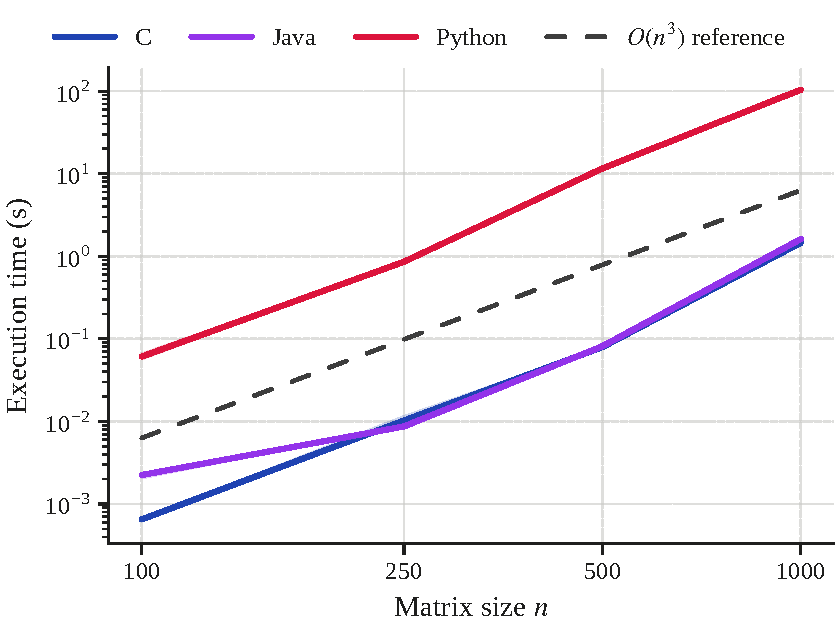
\includegraphics[width=\columnwidth]{time_vs_size.pdf}
  \caption{Median kernel execution time over five runs as a function of the
           matrix size $n$ (log-log). Shaded bands show the interquartile range;
           they are narrow because run-to-run variation was small. The dashed
           line has slope~3 ($\propto n^3$); only its slope, not its height, is
           meaningful.}
  \label{fig:time}
\end{figure}

\begin{figure}[t]
  \centering
  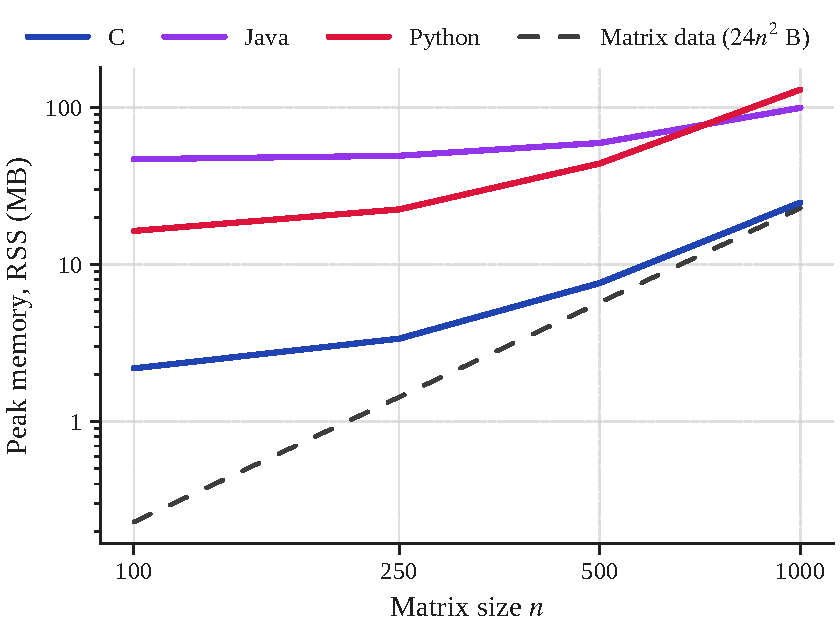
\includegraphics[width=\columnwidth]{memory_vs_size.pdf}
  \caption{Median peak resident set size over five runs as a function of $n$
           (log-log), with interquartile-range bands. The dashed line is the
           size of the three matrices, $24n^2$ bytes.}
  \label{fig:memory}
\end{figure}

\begin{table}[t]
  \centering
  \caption{Median and interquartile range (IQR) over five runs}
  \label{tab:summary}
  \footnotesize
  \setlength{\tabcolsep}{4.5pt}
  % Values computed from results/measurements.csv (same statistics as results_summary.md).
  \begin{tabular}{@{}rlrrrr@{}}
    \toprule
    & & \multicolumn{2}{c}{\textbf{Time (s)}} & \multicolumn{2}{c}{\textbf{Peak RSS (MB)}} \\
    \cmidrule(lr){3-4} \cmidrule(l){5-6}
    $n$ & Language & Median & IQR & Median & IQR \\
    \midrule
    100  & C      & 0.0006500 & 0.000064 & 2.18 & 0.00 \\
         & Java   & 0.002244 & 0.00036 & 46.84 & 0.15 \\
         & Python & 0.06095 & 0.012 & 16.37 & 0.24 \\
    \midrule
    250  & C      & 0.01024 & 0.0020 & 3.37 & 0.06 \\
         & Java   & 0.008692 & 0.00039 & 49.28 & 0.11 \\
         & Python & 0.8577 & 0.033 & 22.43 & 0.20 \\
    \midrule
    500  & C      & 0.07945 & 0.0016 & 7.62 & 0.00 \\
         & Java   & 0.08135 & 0.0019 & 59.45 & 0.01 \\
         & Python & 11.57 & 1.3 & 43.99 & 0.15 \\
    \midrule
    1000 & C      & 1.456 & 0.016 & 24.80 & 0.07 \\
         & Java   & 1.614 & 0.067 & 99.55 & 0.12 \\
         & Python & 103.8 & 2.3 & 130.08 & 0.26 \\
    \bottomrule
  \end{tabular}
\end{table}

\begin{table}[t]
  \centering
  \caption{Empirical time-scaling exponent (model: 3)}
  \label{tab:exponents}
  \footnotesize
  % Least-squares slope of log(median time) vs. log(n), from results/measurements.csv.
  \begin{tabular}{@{}lcc@{}}
    \toprule
    Language & Exponent $b$ & Sizes used \\
    \midrule
    C      & 3.30 & 100--1000 \\
    Java   & 2.84 & 100--1000 \\
    Python & 3.27 & 100--1000 \\
    \bottomrule
  \end{tabular}
\end{table}

\subsection{Execution Time}
Fig.~\ref{fig:time} shows two clearly separated groups. Python is the slowest
language at every size, by a factor of 71 to 146 with respect to C: its median
kernel time grows from 0.061~s at $n=100$ to 103.8~s at $n=1000$. C and Java
are close to each other over most of the range. At $n=100$, Java needs 2.24~ms
against 0.65~ms for C, i.e.\ 3.5 times longer. From $n=250$ onwards the gap
closes: Java is 15\% faster than C at $n=250$ (8.7 vs.\ 10.2~ms), 2\% slower at
$n=500$ (81.4 vs.\ 79.4~ms) and 11\% slower at $n=1000$ (1.61 vs.\ 1.46~s).

All three curves run approximately parallel to the $n^3$ reference line, with
fitted exponents of 3.30 (C), 2.84 (Java) and 3.27 (Python)
(Table~\ref{tab:exponents}). The growth is not uniform across the range,
however. Between consecutive sizes, the cubic model predicts time factors of
15.6 ($100 \to 250$) and 8 ($250 \to 500$ and $500 \to 1000$). C follows the
model closely up to $n=500$ (factors 15.8 and 7.8), but its time grows by 18.3
from $n=500$ to $n=1000$. Java shows the same jump at the same step (19.8).
Python grows faster than cubic one step earlier (13.5 from $n=250$ to $n=500$)
and close to cubic afterwards (9.0).

Run-to-run variation was small. For $n \ge 500$, the IQR is at most 4.1\% of
the median, except for Python at $n=500$ (11\%). It reaches up to 20\% of the
median only for kernels shorter than about 0.1~s, which are the most sensitive
to transient effects.

\subsection{Memory Usage}
Fig.~\ref{fig:memory} shows that the three languages differ mainly in their
baseline (throughout this report, 1~MB $= 2^{20}$ bytes). C has the smallest
footprint at every size: its peak RSS grows from 2.18~MB at $n=100$ to
24.80~MB at $n=1000$, close to the 22.89~MB occupied by the three matrices.
Between $n=500$ and $n=1000$, its RSS grows by 17.2~MB, the same amount as
the matrix data (17.2~MB). Java starts from a large, almost constant baseline
(46.84~MB at $n=100$, 49.28~MB at $n=250$) and reaches 99.55~MB at $n=1000$.
Python starts lower than Java (16.37~MB at $n=100$) but grows much faster, and
overtakes Java between $n=500$ and $n=1000$, reaching 130.08~MB. From $n=500$
to $n=1000$, Java's RSS grows 2.3 times and Python's 5.0 times as much as the
matrix data. Memory measurements were very stable: the largest IQR is
0.26~MB.

% =============================================================================
\section{Discussion}
\label{sec:discussion}
% =============================================================================

\subsection{Empirical Scaling versus the \texorpdfstring{$\bigO{n^3}$}{O(n\textthreesuperior)} Model}
All three implementations grow approximately as $n^3$: on the log-log plot their
curves are nearly straight and roughly parallel to the reference line, and the
fitted exponents (Table~\ref{tab:exponents}) are close to~3. The algorithmic
model therefore correctly predicts the dominant trend. The deviations from it
are, however, systematic and informative.

For C and Python the exponent is \emph{above}~3 (3.30 and 3.27). The
step-by-step factors in Section~\ref{sec:results} show that this excess is not
spread over the whole range but concentrated in one step for each language. C
and Java follow the cubic model up to $n=500$, but when $n$ doubles from 500 to
1000 their time grows by a factor of 18--20 instead of~8. This is consistent
with the access pattern analysed in Section~\ref{sec:background}, and the
thresholds can be checked against the cache sizes of the tested CPU
(Table~\ref{tab:environment}: 48~KB of L1 data cache per core, 8~MB of shared
L3). Reading a column of $B$ touches $n$ different cache lines, i.e.\ $64n$
bytes: about 31~KB for $n=500$, which fits in the L1 data cache, but 62~KB for
$n=1000$, which does not. At the same time, $B$, which is read in full once for
every row of $C$, grows from 1.9 to 7.6~MB, close to the size of the L3 cache
that it shares with $A$ and $C$. Both limits are crossed in exactly the step
where C and Java (which use the same layout) slow down. Beyond these limits,
cache lines can no longer be reused between consecutive iterations, so each
operation waits longer for its data, which an operation-count model does not
capture.

Python reaches this point one step earlier: its time grows 13.5 times from
$n=250$ to $n=500$. Each element is an 8-byte pointer to a separately allocated
24-byte \code{float} object (Section~\ref{sec:disc-memory}), so the same
quantities are four times larger. A column of $B$ touches about two cache lines
per element (one for the pointer, one for the object), i.e.\ about 31~KB at
$n=250$ and 62~KB at $n=500$, and $B$ occupies $32n^2$ bytes, 1.9~MB at
$n=250$ and 7.6~MB at $n=500$. Python therefore crosses the same two cache
limits as C, but between $n=250$ and $n=500$, which is where it slows down.

For Java the exponent is \emph{below}~3 (2.84). This is caused by the smallest
size. At $n=100$ the Java kernel takes 2.24~ms, 3.5 times longer than C
(0.65~ms), and its time then grows only 3.9 times up to $n=250$, where the
model predicts 15.6. From $n=250$ onwards, Java is between 15\% faster and 11\%
slower than C, and it shows the same jump between $n=500$ and $n=1000$ as C.
At $n=100$ the kernel lasts about two milliseconds, so the measurement is
sensitive to effects that do not scale with $n^3$. The most likely candidate is
JIT compilation timing. The three warm-up runs at this size take only a few
milliseconds in total, which may be less than the time the JIT needs to finish
its optimizing (C2) compilation of the kernel in background threads. The timed
run would then still execute less-optimized code. At larger sizes, the warm-up
lasts long enough. A slow first point flattens the fitted slope.

These deviations are hypotheses consistent with the data, not measured facts.
They could be confirmed with hardware performance counters (cache misses per
operation, e.g.\ with \code{perf stat}) or, for Java, by logging JIT activity
with \code{-XX:+PrintCompilation}.

\subsection{Interpreter versus JIT versus Ahead-of-Time Compilation}
The largest effect is the constant factor between execution models: Python is
71 to 146 times slower than C, depending on $n$ (71 times at $n=1000$). Since
all three programs perform the same $2n^3$ operations, this ratio measures the
cost of executing \emph{one} iteration of the inner loop. It is not constant
because the cache effects discussed above affect the two languages at
different sizes: the ratio peaks at $n=500$, where Python has already outgrown
the caches and C has not yet. In C, an iteration is a few machine
instructions: two address computations, two loads, a multiplication and an
addition. In CPython, the same line is executed as a sequence of bytecode
instructions. Each one is dispatched by the interpreter loop and checks the
types of its operands at run time. Index arithmetic on Python integers, list
lookups that return pointers to \code{float} objects, and a multiplication and
an addition that may each create a new \code{float} object, together cost
tens to hundreds of machine instructions.

Java demonstrates what a JIT compiler can achieve: after warm-up, the HotSpot C2
compiler produces native code for the kernel whose speed is within 15\% of
\code{gcc -O2} for $n \ge 250$; at $n=250$ it is even 15\% faster. The
remaining differences come from Java's
safety guarantees (array bounds checks, some of which the JIT can eliminate)
and from differences in code generation. Note that this comparison concerns
\emph{steady-state kernel time}. Java's total run time, including JVM start-up
and warm-up, is larger, and so is its memory footprint (next subsection).

\subsection{Memory Usage and Layout}
\label{sec:disc-memory}
Peak RSS reflects both the matrices and the runtime that holds them.
\emph{C} has almost no runtime overhead. Its RSS is a baseline of about 2~MB
(2.18~MB at $n=100$) plus the matrices. At $n=1000$ it reaches 24.80~MB, only
8\% above the theoretical 22.89~MB of $24n^2$ bytes, and from $n=500$ to
$n=1000$ it grows by exactly the size of the added matrix data.
\emph{Java} starts from a much larger baseline (46.84~MB at $n=100$): the JVM,
its JIT compiler, class metadata and the garbage-collected heap. On top of the
three \code{double[]} arrays, the Java program also holds the input file as a
byte array while it decodes it, which adds $16n^2$ bytes at its peak. Arrays
plus buffer amount to $40n^2$ bytes, 1.7 times the matrix data, while the
measured growth from $n=500$ to $n=1000$ is 2.3 times. The rest is likely
headroom that the garbage collector reserves beyond the live data.
\emph{Python} stores each element as an 8-byte pointer to a 24-byte \code{float}
object, i.e.\ 32 bytes per element instead of~8, so its matrices alone should
take four times the raw size. The measured growth from $n=500$ to $n=1000$ is
even larger, 5.0 times the raw data, the difference being likely due to the
memory allocator's own overhead. Python overtakes Java between $n=500$ and
$n=1000$ and reaches 130.08~MB at $n=1000$, 5.7 times the size of the data.
The memory layout thus affects not only memory use but also speed, through the
cache effects discussed above.

\subsection{Limitations and Threats to Validity}
\begin{itemize}[itemsep=1pt]
  \item \textbf{Single machine.} All results come from one machine
        (Table~\ref{tab:environment}). Cache sizes, memory bandwidth, CPU
        microarchitecture and software versions all affect the results.
        The measurements ran under WSL~2, a virtualized Linux environment,
        which may add overhead compared with native Linux.
  \item \textbf{Frequency scaling and background activity.} Turbo boost,
        thermal throttling and background processes can affect individual
        runs; a few runs took up to twice the median (e.g.\ one C run at
        $n=500$: 0.154~s against a median of 0.079~s). Medians and IQRs reduce
        but do not eliminate these effects.
  \item \textbf{Heterogeneous cores.} The CPU combines one Zen~5 core (up to
        4.5~GHz) with three Zen~5c cores (up to 3.4~GHz). The benchmark is
        single-threaded and was not pinned to a core: under WSL~2, the Windows
        scheduler decides on which physical core each virtual CPU runs. A run
        may therefore execute on either core type, with a difference of about
        25\% in maximum clock. Differences of this order between languages at
        a single size, such as Java being 15\% faster than C at $n=250$,
        should not be over-interpreted.
  \item \textbf{Short kernels.} At $n=100$, the C and Java kernels last
        0.65 and 2.24~ms, which makes them sensitive to short-lived effects
        (cache state, frequency changes, JIT state); their IQRs reach 10--16\%
        of the median.
  \item \textbf{Limited set of sizes.} Only four sizes were tested, so each
        slowdown discussed above is only located between two measured sizes;
        intermediate sizes would be needed to find where it starts. The
        largest size, $n=1000$, was chosen so that the slowest language
        completes within the time budget.
  \item \textbf{Configuration choices.} Results are specific to \code{-O2},
        three Java warm-up runs and the i-j-k loop order. Other choices (e.g.\
        \code{-O3 -march=native}, more warm-up, the cache-friendlier i-k-j order)
        would give different results.
\end{itemize}

% =============================================================================
\section{Conclusions}
\label{sec:conclusions}
% =============================================================================
We implemented the textbook $\bigO{n^3}$ matrix multiplication in C, Java and
Python with identical algorithms, data types, memory layouts and inputs, and
measured its execution time and peak memory for $n$ from 100 to 1000. On the
tested machine (an AMD Ryzen AI 5 330 laptop with 32~GB of RAM, running
Ubuntu 26.04 under WSL~2 on Windows~11) and with the tested settings (GCC 15.2.0
with \code{-O2}, OpenJDK 25.0.4.1 with three warm-up runs, CPython 3.14.4), we
conclude that:
\begin{enumerate}[itemsep=1pt]
  \item \textbf{Time} grows approximately as $n^3$ in all three languages
        (exponents 3.30, 2.84 and 3.27 for C, Java and Python). The deviations
        are concentrated at specific sizes: C and Java slow down faster than
        the model between $n=500$ and $n=1000$, Python between $n=250$ and
        $n=500$. In both cases this is the step in which a column of $B$
        outgrows the 48~KB L1 data cache and $B$ itself approaches the size of
        the 8~MB L3 cache, which is consistent with cache misses causing the
        slowdown.
  \item \textbf{The execution model dominates the constant factor.} The
        interpreted Python version was 71 to 146 times slower than C (71 times
        at $n=1000$). The JIT-compiled Java version was within 15\% of C from
        $n=250$ onwards, but 3.5 times slower at $n=100$, where the kernel
        lasts only milliseconds.
  \item \textbf{Memory} grows as $n^2$ plus a runtime-dependent baseline. C
        stays close to the size of the data (24.80~MB for 22.89~MB of matrices
        at $n=1000$). Java pays a large fixed cost for the JVM (about 47~MB at
        $n=100$). Python needs 5.7 times the data size at $n=1000$ because
        every number is a separate object.
\end{enumerate}
These conclusions apply only to the hardware, software versions and settings
described here. They do not imply that one language is faster in general:
optimized libraries, other compilers, other loop orders or other machines could
change both the absolute numbers and the ranking.

% =============================================================================
\section*{References and Materials}
\addcontentsline{toc}{section}{References and Materials}
% =============================================================================

\paragraph{Materials} All source code, raw measurements and analysis scripts
are available in the public repository linked on the first page. The
main files are:
\begin{itemize}[itemsep=0pt, topsep=2pt, leftmargin=1.2em]
  \item \code{common/data\_generator.py}: shared input generator;
  \item \code{assignment\_1/src/}: the C, Java and Python implementations;
  \item \code{assignment\_1/verify\_correctness.py}: correctness checks;
  \item \code{assignment\_1/run\_benchmark.py}: benchmark harness;
  \item \code{assignment\_1/plot\_results.py}: statistics and figures;
  \item \code{assignment\_1/results/measurements.csv}: raw data;
  \item \code{assignment\_1/README.md}: exact commands to reproduce every
        result in this report.
\end{itemize}

\clearpage

% The bibliography's own heading is suppressed: it lives under the section above.
\begingroup
\renewcommand{\section}[2]{}
\begin{thebibliography}{99}

\bibitem{strassen1969}
V.~Strassen, ``Gaussian elimination is not optimal,''
\emph{Numerische Mathematik}, vol.~13, no.~4, pp.~354--356, 1969.

\bibitem{goto2008}
K.~Goto and R.~A. van~de~Geijn, ``Anatomy of high-performance matrix
multiplication,'' \emph{ACM Transactions on Mathematical Software}, vol.~34,
no.~3, art.~12, 2008.

\bibitem{hennessy2017}
J.~L. Hennessy and D.~A. Patterson, \emph{Computer Architecture: A Quantitative
Approach}, 6th~ed. Cambridge, MA, USA: Morgan Kaufmann, 2017.

\bibitem{drepper2007}
U.~Drepper, ``What every programmer should know about memory,'' Red Hat, Inc.,
Tech. Rep., 2007.

\bibitem{lam1991}
M.~D. Lam, E.~E. Rothberg, and M.~E. Wolf, ``The cache performance and
optimizations of blocked algorithms,'' in \emph{Proc. 4th Int. Conf. on
Architectural Support for Programming Languages and Operating Systems
(ASPLOS)}, 1991, doi:~10.1145/106972.106981.

\bibitem{paleczny2001}
M.~Paleczny, C.~Vick, and C.~Click, ``The Java HotSpot server compiler,'' in
\emph{Proc. USENIX Java Virtual Machine Research and Technology Symposium
(JVM~'01)}, 2001.

\bibitem{georges2007}
A.~Georges, D.~Buytaert, and L.~Eeckhout, ``Statistically rigorous Java
performance evaluation,'' in \emph{Proc. 22nd ACM SIGPLAN Conf. on
Object-Oriented Programming, Systems, Languages and Applications (OOPSLA)},
2007, pp.~57--76.

\bibitem{kalibera2013}
T.~Kalibera and R.~Jones, ``Rigorous benchmarking in reasonable time,'' in
\emph{Proc. ACM SIGPLAN Int. Symp. on Memory Management (ISMM)}, 2013,
pp.~63--74, doi:~10.1145/2464157.2464160.

\bibitem{ieee754}
\emph{IEEE Standard for Floating-Point Arithmetic}, IEEE Std 754-2019, 2019.

\bibitem{higham2002}
N.~J. Higham, \emph{Accuracy and Stability of Numerical Algorithms}, 2nd~ed.
Philadelphia, PA, USA: SIAM, 2002.

\end{thebibliography}
\endgroup

% =============================================================================
\balance
\section*{AI Usage Disclosure}
\addcontentsline{toc}{section}{AI Usage Disclosure}
% =============================================================================
% TODO: Adjust this statement so that it describes exactly how you used AI
%       tools, as required by the course policy.
Generative AI tools were used to support the development of this assignment. Gemini (Google) was used for high-level project planning, repository structuring, and ensuring compliance with the assignment rubric. Claude (Anthropic) was used to draft the initial source code (C, Java, Python), the automated benchmarking and plotting scripts, and the LaTeX report template. 

All AI-generated code and text were thoroughly reviewed, tested, and adapted by the author. The author remains fully responsible for understanding the implementations, executing the experiments on local hardware, validating the measurements, and ensuring the mathematical and factual correctness of every statement in this report.

\end{document}
